% !TEX encoding = UTF-8 Unicode
\documentclass{sig-alternate}
\usepackage{textcomp}
\usepackage{graphics}
\usepackage[utf8]{inputenc}
\usepackage[T1]{fontenc}
\usepackage{listings}
\usepackage{subfigure}

\hyphenation{o-pe-ra-do-res}

\begin{document}

\pagenumbering{arabic}

\title{Algoritmos Genéticos}
\subtitle{Sistemas de Inteligencia Artificial - ITBA}

\numberofauthors{3}

\author{
	\alignauthor{Carlos Sessa}\\
	\alignauthor{Lucas Pizzagalli}\\
	\alignauthor{Nicolás Purita}\\	
}

\date{12 de Junio de 2012}

\maketitle

% \section{Introducción}

% 	Se implementa un motor de algoritmos genéticos para obtener los pesos para la red neuronal construida en el Trabajo Práctico Especial Número 2.
% 	La red neuronal resuelve la función que se puede observar en la figura \ref{fig:function}.

% 	\begin{figure}[!ht]
% 		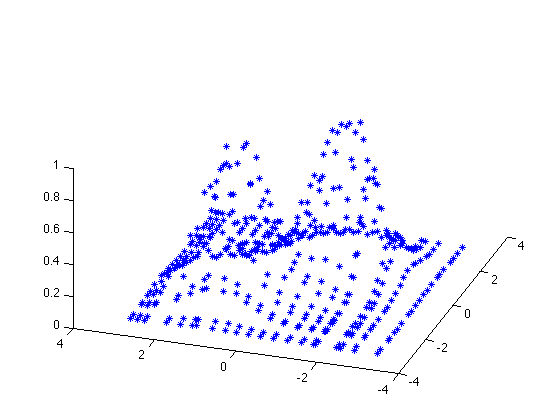
\includegraphics[scale=0.5]{./figures/function.png}
%   		\caption{Distribución de puntos dada}
%   		\label{fig:function}
% 	\end{figure}

% 	En la figura \ref{fig:function} se puede observar que los puntos de la entrada pertenecen al intervalo $[-3.5, 3.5]$ y la salida se encuentra en el intervalo $(0, 1)$.\\
% 	El algoritmo genético se implementó en \textit{Java} y la red neuronal fue realizada en \textit{Matlab}. Utilizando el \textit{MATLAB Compiler Runtime} se realizan las pruebas pertinentes para verificar el funcionamiento de la red.\\

% \section{Desarrollo y Problemas encontrados}

% Se han implementado varios operadores genéticos, métodos de selección, condiciones de corte y demás configuraciones que se presentarán en las secciones a continuación.
% Con el objetivo de facilitar la configuración se ha creado un archivo de \textit{properties} en el que se debe detallar como se desea entrenar la red.
% Un ejemplo de dicho archivo se puede observar en la lista \ref{code:simple}.

% 	\subsection{Operadores genéticos}

% 	\subsubsection{Mutación}
% 	Las mutaciones se realizan tomando un número aleatorio definido entre $-1.5$ y $1.5$.
% 	Se han implementado las mutaciones del tipo clásicas y no uniformes.

% 	\subsubsection{Crossover}
% 	Se han decidido implementar los siguientes algoritmos de cruzamiento:
% 	\begin{itemize}
% 		\item cruce de un punto (clásica)
% 		\item cruce de dos puntos
% 		\item cruce anular
% 		\item cruce uniforme parametrizado
% 		\item Gene
% 	\end{itemize}

% 	\subsubsection{Backpropagation}
% 	Otro operador utilizado es \textit{Backpropagation}.

% 	El mismo toma como parámetro la cantidad de épocas que debe entrenar la red y la probabilidad con la que se debe aplicar.

% 	\subsection{Métodos de selección y reemplazo}

% 	Para ambos casos se han desarrollado los métodos descriptos a continuación, los cuales pueden ser combinados:
	
% 	\begin{itemize}
% 		\item Método de Elitismo
% 		\item Método de Ruleta
% 		\item Método de Torneos
% 		\item Método de Boltzman
% 		\item Método de selección universal estocástica
% 	\end{itemize}

% 	\subsection{Distintas arquitecturas}

% 	Mediante el archivo de configuración se puede seleccionar la arquitectura que se desea utilizar para realizar las pruebas. Las arquitecturas a elegir son las siguientes:

% 	\begin{center}
% 		\begin{enumerate}
% 			\item $[30\,\,20\,\,10\,\,1]$
% 			\item $[10\,\,10\,\,1]$
% 			\item $[10\,\,\,1]$
% 			\item $[10\,\,10\,\,10\,\,10\,\,1]$
% 			\item $[40\,\,20\,\,1]$
% 			\item $[10\,\,10\,\,10\,\,1]$
% 			\item $[5\,\,10\,\,20\,\,1]$
% 		\end{enumerate}
% 	\end{center}

% 	\subsection{Representación del individuo}

% 	Con el objetivo de representar al individuo, se ha elegido transformar
% 	la matriz de pesos a un vector de números \textit{doubles} como se muestra en
% 	la figura \ref{fig:indiv} y de esta forma poder aplicar los operadores
% 	pertinentes de una forma rápida y sencilla. \\

% 	Esta representación no se adapta a la representación de la matriz en
% 	\textit{MATLAB}, por lo tanto se realiza una transformación del individuo.
% 	Esta transformación consiste en cambiar el vector de doubles por una
% 	matriz y viceversa. \\

% 	\subsubsection{Fidelidad del individuo}

% 	\begin{itemize}

% 		\item \textbf{Completitud}: Es completa ya que se puede representar todo el dominio del problema.

% 		\item \textbf{Coherencia}: Representa únicamente el dominio del problema, ya que ninguna representación puede pertenecer a un conjunto fuera del dominio.

% 		\item \textbf{Uniformidad}: Se puede concluir que esta representación es uniforme ya que es imposible representar dos individuos distintos con la misma cadena, en caso que esto sucediera esa representación sería exactamente la misma que la otra.	

% 		\item \textbf{Sencillez}: Convertir matriz de pesos a un vector de doubles es una operación simple.

% 		\item \textbf{Localidad}: Es local dada que un cambio en un elemento
% 		del vector genera un cambio en el peso de la conexión que representa.

% 	\end{itemize}

	\section{Consideraciones generales}

		\subsection{Cálculo del Fitness}

			El fitness del individuo es obtenido mediante una simple división del \textit{Error cuadrático medio} que se obtiene de la red al evaluar los puntos.
			La fórmula para el mismo es:

			\begin{equation}
				\textbf{Fitness} = \dfrac{1}{ECM}
			\end{equation}

			donde \textit{ECM} es el Error Cuadrático Medio.

		\subsection{Selección de valores para Boltzman}

			Para elegir los valores iniciales de las temperaturas que se utilizan en el algoritmo de Boltzman (Temperatura mínima, máxima y decremento por generación) se eligieron ciertos valores que cumplan con el siguiente criterio. Al inicio de la evolución todos los individuos deben tener una probabilidad similar de ser seleccionados entre toda la población y a medida que avanzan las generaciones los individuos con mayor \textit{fitness} deben tener mayor probabilidad de ser seleccionados.
			Los valores que se eligieron de Boltzman para hacer las pruebas son variables dependiendo de la cantidad de iteraciones que se desea realizar, y suponiendo un \textit{fitness} en un rango determinado. Esto logra una gran diversidad en un comienzo, y luego va refinando la población descartando de a poco las opciones malas. 	

	\section{Resultados y Conclusiones}

		Con el fin de obtener resultados comparables entre sí se define un
		contexto base para todas las pruebas, con la intención de obtener distintos 
		resultados se realizan cambios sobre esta configuración:

		\begin{itemize}
			\item \textbf{Cantidad de individuos:} 52.
			\item \textbf{Mutación:} Clásica. Con una probabilidad de mutar un individuo de $0.5$ 
			y de mutar un locus de $0.03$ donde tenemos una probabilidad de $0.015$ de mutar.
			\item \textbf{Cruce:} Clásico.
			\item \textbf{Backpropagation:} 0 (Desactivado)
			\item \textbf{Selección:} Elite+Rulette (Seleccionando 5 para Elite y 23 para Rulette).
			\item \textbf{Reemplazo:} Elite+Rulette (Seleccionando 6 para Elite y 18 para Rulette).
			\item \textbf{Criterios de corte:} Máxima 500 generaciones o Contenido, si en 60 generaciones
			no mejora un $1\%$ el mejor individuo corta.
		\end{itemize}

		\subsection{Backpropagation vs Algorítmo Genéticos con Backpropagation}


		En las figuras \ref{fig:onlyBP} y \ref{fig:AGWithBP} se puede observar como mejora la \textit{Red neuronal} utilizando Algorítmos Genéticos. El primer punto a destacar es el comportamiento de la curva del \textit{Fitness}, en la figura \ref{fig:AGWithBP} se puede observar que se obtiene un mejor resultado que la figura \ref{fig:onlyBP} y además no posee esas oscilaciones que presenta la red al utilizar método Batch como corrección. Se puede observar que los dos algoritmos mejoran a traves del tiempo, sólo que en la figura \ref{fig:AGWithBP} lo hace con mayor velocidad.
		
		\subsection{Boltzman}

		Con el objetivo de analizar el desempeño de este método de selección y reemplazo, se decidió probar con una configuración Boltzman-Boltzman (donde la selección y el reemplazo se realiza con dicho método) con una configuración como la siguiente:
			
		\begin{enumerate}			
			\item \textit{Temperatura inicial}: 50
			\item \textit{Temperatura mínima}: 0.5
			\item \textit{Decremento por generación}: 0.5
			\label{eq:boltz}
		\end{enumerate}

		Esto quiere decir que la temperatura mínima se alcanza en 100 generaciones aproximadamente, 	o sea que entre la primera y la generación número 100, se van seleccionando cada vez más proporción de individuos con \textit{fitness} más alto.\\
		Como se puede observar en la figura \ref{fig:boltzboltz}, tanto el valor medio como el mejor \textit{fitness} tienden a empeorar, comportarse de una forma bastante errática y luego comenzar a mejorar de a poco. Esto se debe a que, como se ha descripto anteriormente, en un comienzo se tiende a elegir de una manera casi totalmente aleatoria, pero a medida que se acerca y supera la generación 100 y se alcanza la temperatura mínima, la selección se realiza más a conciencia, dándole prioridad a los individuos con más aptitud. 
		
		\subsection{Mutación No uniforme}
		
		Con el objetivo de comparar el comportamiento del sistema según como varía el decaimiento de la probabilidad de mutación a medida que las generaciones avanzan. Por lo tanto, se decidió comparar mutaciones no uniformes con decaimientos de $5\%$, $10\%$ y $15\%$ cada 30 generaciones. Los resultados se las mismas se pueden observar en las figuras \ref{fig:mut_no_un_5} , \ref{fig:mut_no_un_10} y \ref{fig:mut_no_un_15} respectivamente. De las mismas se puede observar a simple vista, como en todos los casos termina por contexto (60 generaciones con un cambio menor a $1\%$), sin embargo, se puede ver como al ser el decremento mayor, el algoritmo termina antes. Esto se debe a que al haber muchas menos mutaciones, no hay introducción de elementos nuevos y no se llega a cambiar lo suficiente las redes como para obtener nuevas combinaciones y se consigan mejores resultados. Este estancamiento, también se evidencia en el menor desvío estándar.

		\subsection{Crossover}
		Se prueban distintas opciones de crossover.
		Los resultados se pueden ver en la figura \ref{fig:crossover_comparison}.
		Se puede observar en la figura \ref{fig:crossover_anular} que es el método
		que llega al mejor fitness.

% \section{Posibles mejoras}

% \subsection{Mejoras a backpropagation}
% 	Como posible mejora se concluye que el operador \textit{backpropagation}
% 	podría disminuir su probabilidad de acción a medida que se alcanza un
% 	fitness deseado.
% 	El motivo por el cual se desea disminuir esa probabilidad es para que
% 	comience a tener más influencia los operadores de mutación y cruce.
% 	El deseo de que la mutación y cruce tenga más influencia a lo largo de
% 	las generaciones es porque se observó que el fitness en un punto se
% 	asintotiza al error cuadrático medio obtenido por \textit{backpropagation}
% 	en el Trabajo Práctico Especial 2.\\

% \subsection{Mejoras a criterios de selección y reemplazo}
% 	En algunas corridas nos pasó que perdimos al mejor individuo entre
% 	generaciones. Sería conveniente agregar un parámetro a los criterios
% 	de selección y reemplazo para que siempre dejen el individuo con mejor
% 	aptitud.

% \subsection{Mutación evolutiva}
% Se podría probar evolucionar la probabilidad de mutación de cada individuo
% de la población.
% En vez de tomarse una probabilidad de mutación global, se agrega al
% genotipo de cada individuo un gen que codifica la probabilidad
% de mutación del resto del cromosoma.
% En otras palabras, en vez de fijar la probabilidad de mutación
% arbitrariamente, la probabilidad de mutación tiene libertad de
% moverse según mejor le convenga a cada individuo para mejorar su fitness.

% \section{Conclusiones}
% Finalmente, se llega a la conclusión de que, debido a la naturaleza del
% problema que se desea resolver, es necesaria la utilización del
% operador \textit{backpropagation} para llegar a resultados deseados.

% El hecho de correr \textit{backpropagation} generó mejores individuos que
% luego al aplicarle operadores genéticos mejoran notablemente.

\onecolumn


\begin{figure}[!ht]
	\begin{center}
		\subfigure[Únicamente Backpropagation]
			{\label{fig:onlyBP}\framebox{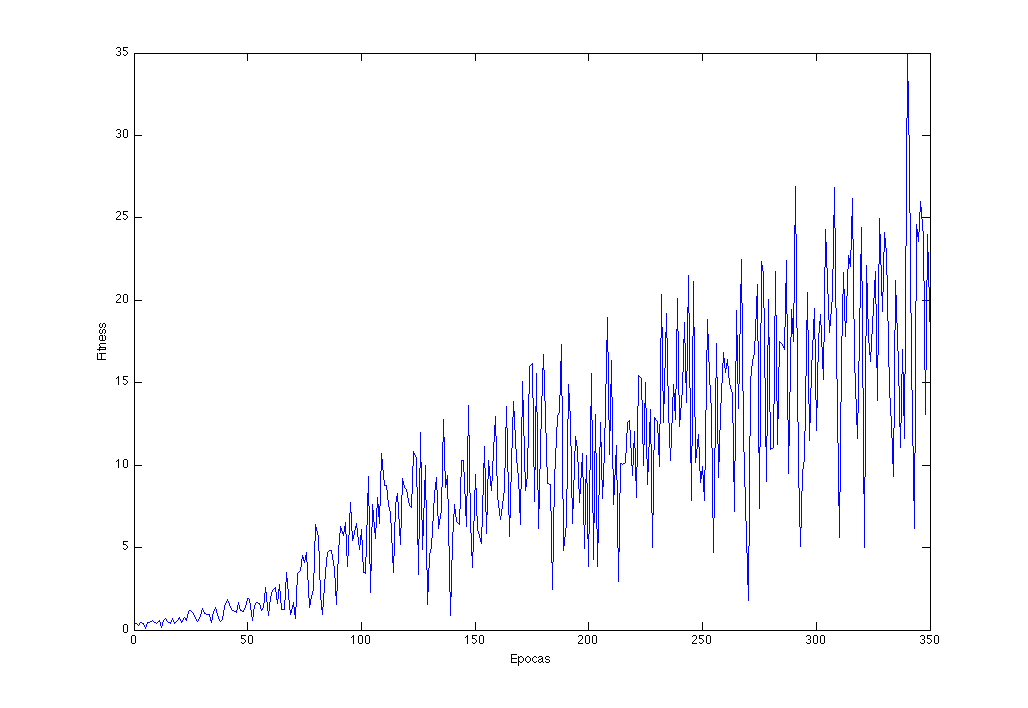
\includegraphics[scale=0.3]{./figures/OnlyBPFitness.png}}}
		\hspace{20pt}
		\subfigure[Algoritmo Genético con Backpropagation]
			{\label{fig:AGWithBP}\framebox{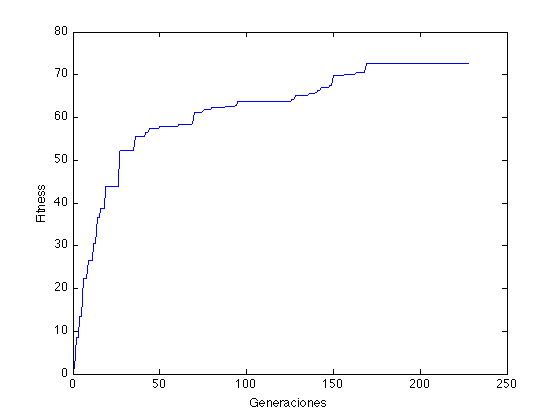
\includegraphics[scale=0.5]{./figures/BPFitness.png}}}
	\end{center}
	\caption{Comparación entre Backpropagation y Algoritmo Genéticos con Backpropagation}
	\label{fig:comparinBP}
\end{figure}

\begin{figure}[!ht]
	\begin{center}
		\hspace{20pt}
		\subfigure[Crossover Classic]
			{\label{fig:crossover_classic}\framebox{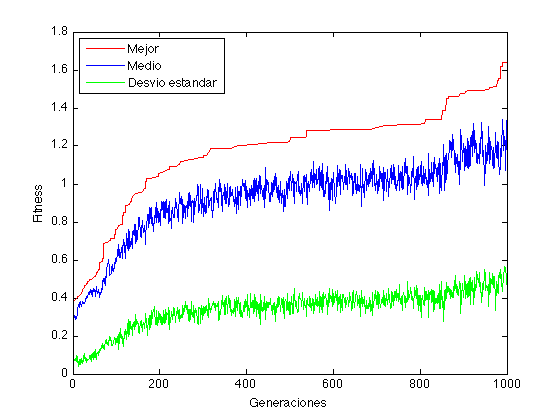
\includegraphics[scale=0.35]{./figures/crossover_classic.png}}}

		\hspace{20pt}
		\subfigure[Crossover Multiple Point con dos puntos]
			{\label{fig:crossover_multipoint}\framebox{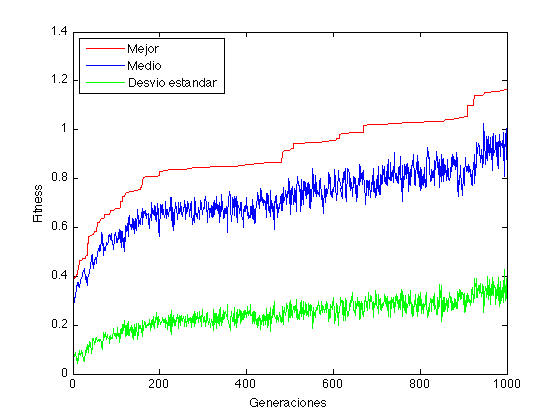
\includegraphics[scale=0.35]{./figures/crossover_multipoint.png}}}

		\hspace{20pt}
		\subfigure[Crossover Uniform]
			{\label{fig:crossover_multipoint}\framebox{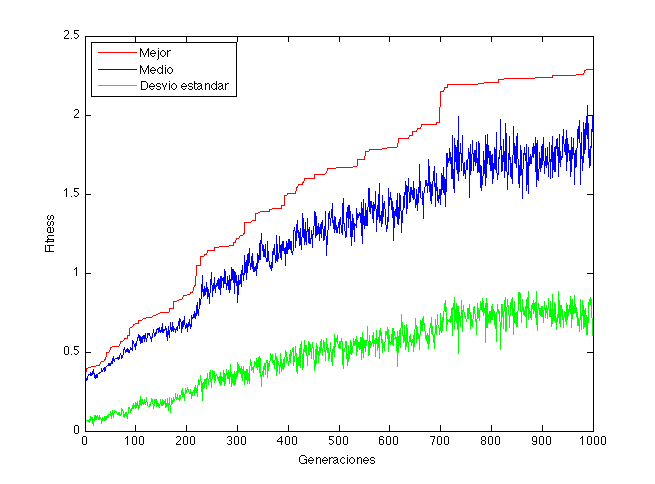
\includegraphics[scale=0.35]{./figures/crossover_uniform.png}}}

		\hspace{20pt}
		\subfigure[Crossover Anular]
			{\label{fig:crossover_anular}\framebox{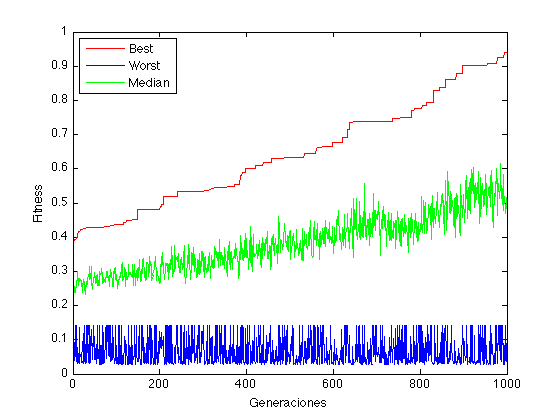
\includegraphics[scale=0.35]{./figures/crossover_anular.png}}}

		\hspace{20pt}
		\subfigure[Crossover Gene]
			{\label{fig:crossover_gene}\framebox{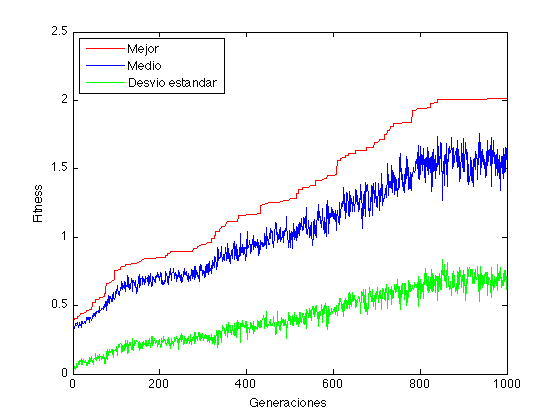
\includegraphics[scale=0.35]{./figures/crossover_gene.png}}}

	\end{center}
	\caption{Comparación entre distintos métodos de crossover}
	\label{fig:crossover_comparison}
\end{figure}


\begin{table}[htp]
	\begin{center}
	\begin{tabular}{|c|c|c|c|}
		\hline
	     Fitness & Generación & Corte & $p_{m}$ \\
		\hline
		0.22501570790437642 & 60 & Contenido & 0.05 \\
		0.21842640558999668 & 60 & Contenido & 0.1 \\
		0.22113522454399956 & 67 & Contenido & 0.3 \\ 
		0.22050756611447994 & 72 & Contenido & 0.5 \\
		\hline
	\end{tabular}
	\caption{Configuración simple variando la $p_m$}
	\label{table:simple_mutation_prob}
	\end{center}
\end{table}

\begin{table}[htp]
	\begin{center}
	\begin{tabular}{|c|c|c|c|c|p{1cm}|}
		\hline
	     Fitness & Generación & Corte & $p_{m}$ & decrecimiento (\%) & dec. gen. \\
		\hline
		0.21222349890474348 & 50 & Content & 0.6 & 5 & 30 \\
		0.22795744299992385 & 77 & Content & 0.6 & 10  & 30 \\
		0.21740760693242447 & 65 & Content & 0.6 & 15 & 30 \\
		\hline
	\end{tabular}
	\caption{Configuración simple método de mutación No Uniforme}
	\label{table:simple_mutation_no_uniform}
	\end{center}
\end{table}

\begin{table}[htp]
	\begin{center}
	\begin{tabular}{|c|c|c|c|c|}
		\hline
	     Fitness & Generación & Corte & $p_{m}$ & Cruce \\
		\hline
		0.22501570790437642 & 60 & Contenido & 0.05 & Clásico \\
		0.20662153685787393 & 50 & Contenido & 0.05 & Gene \\
		0.21418198155450324 & 50 & Contenido & 0.05 & Multiples puntos con 2 \\
		0.21674758534799746 & 70 & Contenido & 0.05 & Uniforme con 0.3 prob \\
		0.20662153685787393 & 50 & Contenido & 0.05 & Anular \\
		\hline
	\end{tabular}
	\caption{Configuración simple variando el método de cruce}
	\label{table:crossover}
	\end{center}
\end{table}

\begin{table}[htp]
	\begin{center}
	\begin{tabular}{|c|c|c|c|}
		\hline
	     Nombre .properties & Fitness & Generación & Corte \\
		\hline
		bp\_seb\_rer\_cg\_mc\_ec.properties 		& 16.720276062651436 	& 69 & Contenido \\
		bp\_ser\_reb\_mc\_cc\_emc.properties 	& 11.941655508072634 	& 58 & Contenido \\
		bp\_se\_re\_mc\_cc\_emc.properties 		& 4.825691593990156 	& 51 & Contenido \\
		bp\_seb\_rer\_cmp\_mc\_emc.properties 	& 12.57897997517028 	& 36 & Contenido \\
		bp\_seb\_rer\_mc\_ca\_emc.properties 	& 13.560979676949982 	& 50 & Contenido \\
		bp\_seb\_rer\_mnu\_cc\_emc.properties 	& 12.992838764610976 	& 36 & Contenido \\
		\hline
	\end{tabular}
	\caption{Distintas Configuraciones con backpropagation}
	\label{table:backpropagation}
	\end{center}
\end{table}

\newpage

\begin{lstlisting}[caption={Archivo de configuración simple},label={code:simple}]

popSize = 52
architecture = 2
generationGap = 0.5

mutation = Classic
mutationProbability = 0.5
Mutation.alleleProb = 0.03

Backpropagation.probability = 0

crossover = Classic
crossoverProbability = 1


selection = Elite / Rulette
Elite.toSelect = 5
Rulette.toSelect = 23

replacement = Elite / Rulette
replacement.Elite.toSelect = 6
replacement.Rulette.toSelect = 18

ending = MaxGeneration / Content
MaxGeneration.iterationToEnd = 500

Content.improvement = 0.01
Content.iterationToImprove = 60
Content.iterationToImprove = 15

\end{lstlisting}


\end{document}
